\documentclass{amsart}
\usepackage[usefamily=sage]{pythontex} 
\usepackage{float}
\usepackage{tikz}
\usetikzlibrary{calc}
\usepackage[utf8]{inputenc}
\usepackage[most]{tcolorbox}
\usepackage[margin = 2cm]{geometry}

\newtheorem{ejer}{Ejercicio}
\def\r{\mathbb{R}}
\title{Tarea 08. Giros en el Plano \\ AMD 2024-25}
\author{Manuel Bernal Hernández}
\begin{document}
\maketitle

\begin{ejer}
Construye la bandera de Chile con la especificaciones indicadas el el siguiente gráfico:

\begin{figure}[H]
\centering
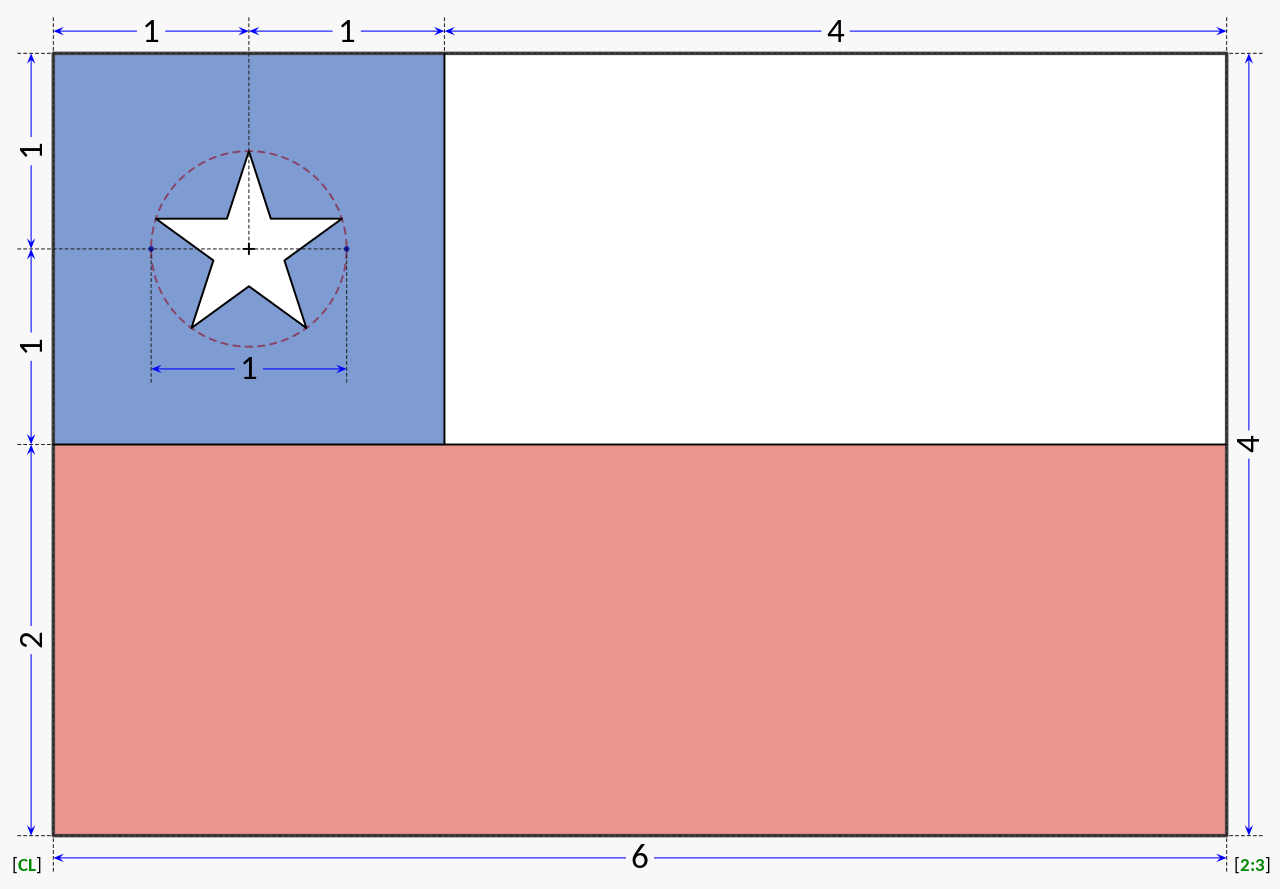
\includegraphics[width = 12cm]{Chile.png}
%(Fuente: \url{https://en.wikipedia.org/wiki/Flag_of_Chile#/media/File:Flag_of_Chile_(construction_sheet).svg})
\end{figure}
\end{ejer}

{\it Solución:}

% Escribe tu solución para el ejercicio 4
\begin{sageblock}

A = vector([3/2, 3/2])
beta = 2*pi/5
G = matrix(RR,[[cos(beta), -sin(beta)], [sin(beta), cos(beta)]])
V = [A+G^i*vector([0,1/2]) for i in range(5)]

\end{sageblock}

\begin{center}
\begin{tikzpicture}[x = 2cm, y = 2cm, baseline=9mm, vertice/.style = {fill=white,circle,draw}, scale=0.6]

\fill[blue] (0,0) rectangle (3,3);
\draw[black] (0,0) rectangle (3,3);
\fill[white] (3,0) rectangle (9,3);
\draw[black] (3,0) rectangle (9,3);
\fill[red] (0,-3) rectangle (9,0);
\draw[black] (0,-3) rectangle (9,0);

%\fill[color=white] !{V[0]} -- !{V[2]} -- !{V[4]} -- !{V[1]} -- !{V[3]} -- !{V[0]} -- cycle;
\fill[color = white] !{V[0]} -- !{V[2]} -- !{V[4]} -- !{V[1]} -- !{V[3]} -- cycle;

\end{tikzpicture}
\end{center}


\end{document}
